\documentclass[10pt,twocolumn,letterpaper]{article}
\usepackage[margin=0.75in,columnsep=0.3in]{geometry}
\usepackage{times}
\usepackage[T1]{fontenc}
\usepackage{microtype}
\usepackage{amsmath,amssymb}
\usepackage{graphicx}
\usepackage{booktabs}
\usepackage{multirow}
\usepackage{array}
\usepackage{xcolor}
\usepackage[font=small,labelfont=bf,skip=4pt]{caption}
\usepackage{enumitem}
\usepackage{listings}
\usepackage{tikz}
\usetikzlibrary{arrows.meta,positioning,fit,calc}
\usepackage[colorlinks=true,linkcolor=black,citecolor=blue!50!black,urlcolor=blue!50!black]{hyperref}
\usepackage{titlesec}
\titleformat{\section}{\normalfont\large\bfseries}{\thesection}{0.6em}{}
\titleformat{\subsection}{\normalfont\normalsize\bfseries}{\thesubsection}{0.6em}{}
\titlespacing*{\section}{0pt}{9pt}{4pt}
\titlespacing*{\subsection}{0pt}{6pt}{3pt}
\setlist{nosep,leftmargin=1.2em}
\lstset{basicstyle=\ttfamily\footnotesize,columns=fullflexible,frame=single,framerule=0.3pt,rulecolor=\color{black!30},backgroundcolor=\color{black!3},xleftmargin=2pt,xrightmargin=2pt,aboveskip=4pt,belowskip=4pt}
\definecolor{nblue}{HTML}{1F5FBF}
\definecolor{nteal}{HTML}{0B7A6E}
\definecolor{norange}{HTML}{C25A1C}
\tikzset{
  box/.style={draw=black!55,rounded corners=2pt,align=center,font=\footnotesize,inner sep=3pt,minimum height=0.85cm,fill=white},
  arr/.style={-{Stealth[length=4pt]},thick,black!65},
  grp/.style={draw=black!35,dashed,rounded corners=4pt,inner sep=5pt}
}

\title{\textbf{ProbTalk3D Studio: Replicating, Evaluating and Deploying\\a Non-Deterministic, Emotion-Controllable Speech-to-3D-Face Model}}
\author{Jyothi Masina \qquad Shruti Deulgaonkar\\[2pt]
\small University of North Carolina at Charlotte\\
\small Course project, Fall 2026\\[2pt]
\small Code: \url{https://github.com/jsdmhash/ProbTalk3D} \quad Project page: \url{https://jsdmhash.github.io/ProbTalk3D/}}
\date{}

\begin{document}
\maketitle

\begin{abstract}
ProbTalk3D (Wu, Haque and Yumak, ACM SIGGRAPH MIG 2024) animates a 3D face from speech with explicit control over emotion and intensity, and produces a different but plausible performance on every run by sampling from a learned motion codebook. We report a three-stage study of this model. First, we trace the released code end to end and identify six reproducibility risks. Second, we replicate inference on current software (Python 3.13, PyTorch 2.11) with three loading patches and no change to the network, and verify both central claims: sampling alone produces take-to-take variation, and a temperature parameter controls its size. Third, we build \emph{ProbTalk3D Studio}, a cloud service with a web studio, a public API, a Python client and an installable phone app, together with a Blender-free renderer that adds eyes, brows and lips to the FLAME head. On 478 ground-truth sequences from 3DMEAD our deployment reproduces the paper's mean vertex error within 2.6\% and its diversity within 4.8\%. A temperature sweep shows that the paper's default ($T{=}0.2$) costs about 1.5\% error relative to deterministic decoding while adding substantial variety. A 25-person user study rates lip-sync at 3.91/5 and recognises emotion from silent clips at 39\%, about three times chance.
\end{abstract}

\section{Introduction}
Speech-driven 3D facial animation turns an audio track into the motion of a 3D face. It is used in games, film, virtual reality and avatar-based communication, where hand animation is slow and expensive. Most published systems are \emph{deterministic}: the same audio always produces the same motion~\cite{faceformer,codetalker}. Real speakers never repeat a sentence identically, and they colour speech with emotion. ProbTalk3D~\cite{probtalk3d} was the first model to offer both explicit emotion control and non-deterministic output in one network.

The model is also interesting from a networking point of view. A 720p video call needs on the order of 4\,Mbps. If the receiver can generate the face, the sender only needs to transmit speech (256\,kbps as raw 16\,kHz, 16-bit PCM, far less once compressed) plus a 43-number style code, which is about 16 times less data even before audio compression. The generated motion itself is only 42\,kbps (53 parameters $\times$ 25 frames $\times$ 4 bytes), and the receiver can choose the emotion.

This report documents our work in three milestones and an evaluation:
\begin{itemize}
\item \textbf{M1, code review:} a traced inference path through the released code and a list of reproducibility risks (Sec.~\ref{sec:m1}).
\item \textbf{M2, replication:} inference on modern software with three minimal patches, and verification of the paper's two claims (Sec.~\ref{sec:m2}).
\item \textbf{M3, deployment:} ProbTalk3D Studio, a client-server service with a new renderer (Sec.~\ref{sec:m3}).
\item \textbf{Evaluation:} ground-truth metrics, a temperature matrix, per-emotion displacement maps and a user study (Sec.~\ref{sec:eval}).
\end{itemize}

\section{Background and Related Work}
\textbf{Deterministic models.} VOCA~\cite{voca} regresses FLAME~\cite{flame} vertex offsets from audio features. FaceFormer~\cite{faceformer} uses a transformer with a pretrained speech encoder, and CodeTalker~\cite{codetalker} casts the problem as code queries into a discrete motion prior learned with a VQ-VAE~\cite{vqvae}. All three map one audio clip to one motion.

\textbf{Non-deterministic models.} FaceDiffuser~\cite{facediffuser} applies diffusion to produce varied motion, and CodeTalker can be made stochastic, but neither exposes an emotion control.

\textbf{Emotion-controllable models.} EMOTE~\cite{emote} and EmoTalk~\cite{emotalk} condition on emotion labels but remain deterministic. EMOTE also introduced 3DMEAD, a FLAME reconstruction of the MEAD audio-visual emotion corpus~\cite{mead}, which ProbTalk3D uses for training.

\textbf{ProbTalk3D}~\cite{probtalk3d} combines a VQ-VAE motion prior with a style-conditioned speech encoder and samples codebook entries at inference time. It reports MVE $0.7243$, LVE $0.6040$ and diversity $0.3274$ on 3DMEAD (scaled units), close to the most accurate baseline while about 4.5 times more diverse, and it was preferred over FaceDiffuser and EMOTE in a 69-person user study.

\section{The ProbTalk3D Model}
\label{sec:model}
\begin{figure*}[t]
\centering
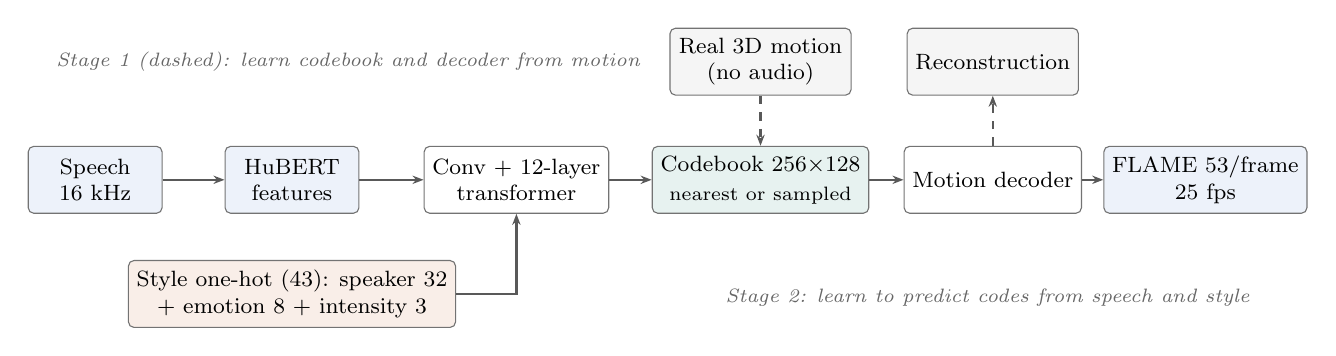
\begin{tikzpicture}
\node[box,fill=nblue!8,minimum width=1.7cm] (aud) at (0,0) {Speech\\16 kHz};
\node[box,fill=nblue!8,minimum width=1.7cm] (hub) at (2.5,0) {HuBERT\\features};
\node[box,minimum width=2.3cm] (enc) at (5.35,0) {Conv + 12-layer\\transformer};
\node[box,fill=nteal!10,minimum width=2.3cm] (cb) at (8.45,0) {Codebook 256$\times$128\\[1pt]\scriptsize nearest or sampled};
\node[box,minimum width=2.1cm] (dec) at (11.4,0) {Motion decoder};
\node[box,fill=nblue!8,minimum width=2.0cm] (out) at (14.1,0) {FLAME 53/frame\\25 fps};
\node[box,fill=norange!10,minimum width=2.9cm] (sty) at (2.5,-1.45) {Style one-hot (43): speaker 32\\+ emotion 8 + intensity 3};
\node[box,fill=black!4,minimum width=2.3cm] (mot) at (8.45,1.5) {Real 3D motion\\(no audio)};
\node[box,fill=black!4,minimum width=2.1cm] (rec) at (11.4,1.5) {Reconstruction};
\draw[arr] (aud) -- (hub);
\draw[arr] (hub) -- (enc);
\draw[arr] (sty.east) -| (enc.south);
\draw[arr] (enc) -- (cb);
\draw[arr] (cb) -- (dec);
\draw[arr] (dec) -- (out);
\draw[arr,dashed] (mot) -- (cb);
\draw[arr,dashed] (dec) -- (rec);
\node[font=\scriptsize\itshape,black!60,anchor=east] at ($(mot.west)+(-0.25,0)$) {Stage 1 (dashed): learn codebook and decoder from motion};
\node[font=\scriptsize\itshape,black!60,anchor=west] at ($(sty.east)+(3.3,-0.05)$) {Stage 2: learn to predict codes from speech and style};
\end{tikzpicture}
\caption{ProbTalk3D's two stages. Stage 1 (dashed) trains a VQ-VAE on 3D motion alone, giving a codebook of 256 real motion entries and a decoder. Stage 2 trains a speech encoder, conditioned on a 43-dimensional style code, to predict codebook entries; the decoder stays frozen. At inference the quantiser either takes the nearest entry or samples one (Eq.~\ref{eq:sample}).}
\label{fig:model}
\end{figure*}

Fig.~\ref{fig:model} summarises the architecture. \textbf{Stage 1} is a motion VQ-VAE trained on 3DMEAD without audio. It learns a codebook $\mathcal{C}=\{c_k\}_{k=1}^{256}$, $c_k\in\mathbb{R}^{128}$, and a decoder from code sequences back to FLAME expression and jaw parameters (50 + 3 values per frame at 25\,fps). \textbf{Stage 2} encodes 16\,kHz speech with HuBERT~\cite{hubert}, concatenates a one-hot style vector $s\in\{0,1\}^{43}$ (32 speakers, 8 emotions, 3 intensities), and passes the result through convolution and a 12-layer transformer to predict one latent $z_t$ per frame, which is quantised against $\mathcal{C}$ and decoded by the frozen Stage-1 decoder.

\textbf{Sampling.} Let $d_{t,k}=\lVert z_t-c_k\rVert^2$. During training, and whenever sampling is disabled, the quantiser picks $\arg\min_k d_{t,k}$. At generation time it instead draws
\begin{equation}
k_t \sim \mathrm{Categorical}\!\left(\mathrm{softmax}\!\left(-d_{t,\cdot}/T\right)\right),
\label{eq:sample}
\end{equation}
so nearer entries are more likely and the temperature $T$ controls how far the choice can wander. In our measurements the nearest entry wins about 95\% of the time at $T{=}0.05$ and only about 21\% at $T{=}1.0$; the paper's default is $T{=}0.2$. Because every entry is a motion learned from real faces, sampled takes stay plausible. In the code this is a single branch in \texttt{vqvae\_quantizer.py}:
\begin{lstlisting}[language=Python]
if not sample:
    idx = torch.argmin(d, dim=1)
else:
    probs = softmax(-d / temperature)
    idx = torch.multinomial(probs, 1)
\end{lstlisting}

\section{Milestone 1: Code Review}
\label{sec:m1}
We traced one inference run through the released repository in six steps: Hydra merges the saved configuration with command-line overrides; \texttt{instantiate()} builds the model from YAML; the checkpoint is loaded in evaluation mode and the temperature set; audio is loaded as normalised 16\,kHz mono; \texttt{model(batch, sample)} returns a tensor of shape $[1,T,53]$; and the output is de-normalised and padded to 403 FLAME parameters per frame. The relevant code lives in \texttt{train\_all.py}, \texttt{generation.py}, \texttt{evaluation.py} (six metrics), \texttt{configs/}, \texttt{framework/} and \texttt{render\_*.py}. Table~\ref{tab:risks} lists the risks we identified before running anything.

\begin{table}[t]
\centering\small
\caption{Reproducibility risks found in the M1 code review and how M2 resolved them.}
\label{tab:risks}
\begin{tabular}{@{}>{\raggedright\arraybackslash}p{3.5cm}>{\raggedright\arraybackslash}p{3.8cm}@{}}
\toprule
Risk & Resolution in M2\\
\midrule
Python 3.9, 182 pinned packages & 38 packages on Python 3.13\\
Bundled HuBERT imports a removed module & Import \texttt{HubertModel} from \texttt{transformers}\\
Checkpoint load fails on PyTorch $\geq$2.6 & Load with \texttt{weights\_only=False}\\
Weight-norm key names changed & Remap \texttt{weight\_g/v} to \texttt{original0/1}\\
Batch size 1 only & Kept; adequate for inference\\
Weights on Google Drive; Blender for rendering & \texttt{gdown}; own renderer in M3\\
\bottomrule
\end{tabular}
\end{table}

\section{Milestone 2: Replication}
\label{sec:m2}
We ran inference on a Colab T4 GPU (15\,GB) with Python 3.13, PyTorch 2.11 and Transformers 5.20. Three patches, each marked \texttt{\# PATCH} in the code, were sufficient (Table~\ref{tab:risks}); the network and its mathematics are unchanged. All eight test clips produced outputs of shape $(1,T,403)$ at 25\,fps, with an audio alignment gap below 0.04\,s and about 2.4\,s of GPU time per clip.

Table~\ref{tab:m2} checks the paper's claims. With sampling on, three runs on identical input differ (mean pairwise parameter difference 0.017). With sampling off, two runs are identical to six decimal places, so the variation comes only from the sampling step. The difference grows monotonically with temperature, 4.7 times from $T{=}0.05$ to $T{=}1.0$.

\begin{table}[t]
\centering\small
\caption{M2 verification of non-determinism and temperature control (mean pairwise difference between takes of the same input, FLAME parameter space).}
\label{tab:m2}
\begin{tabular}{@{}lc@{}}
\toprule
Setting & Take-to-take difference\\
\midrule
Sampling off (2 runs) & 0.000000\\
$T=0.05$ & 0.008\\
$T=0.2$ (paper default, 3 runs) & 0.017\\
$T=0.5$ & 0.027\\
$T=1.0$ & 0.038\\
\bottomrule
\end{tabular}
\end{table}

\section{Milestone 3: ProbTalk3D Studio}
\label{sec:m3}
\begin{figure*}[t]
\centering
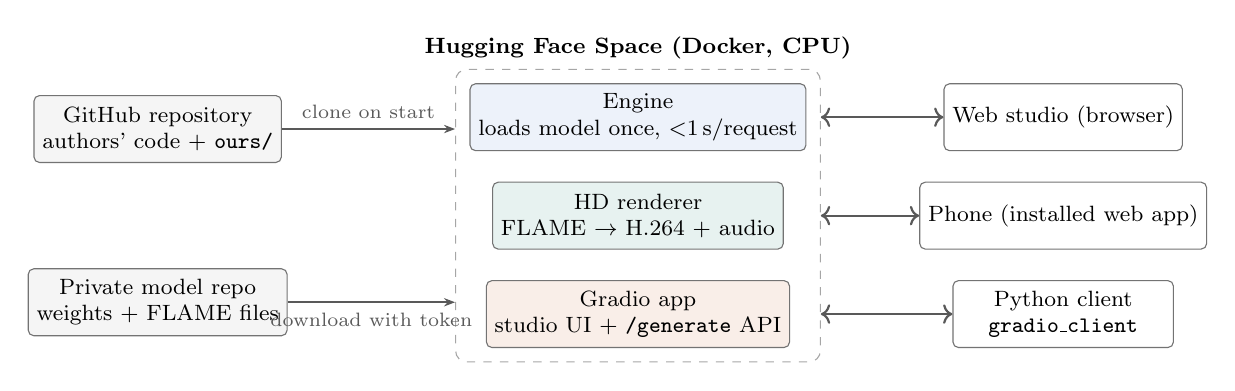
\begin{tikzpicture}
\node[box,minimum width=3.0cm,fill=black!4] (gh) at (0,1.1) {GitHub repository\\authors' code + \texttt{ours/}};
\node[box,minimum width=3.0cm,fill=black!4] (hf) at (0,-1.1) {Private model repo\\weights + FLAME files};
\node[box,minimum width=3.2cm,fill=nblue!8] (eng) at (6.1,1.25) {Engine\\loads model once, $<$1\,s/request};
\node[box,minimum width=3.2cm,fill=nteal!10] (ren) at (6.1,0) {HD renderer\\FLAME $\rightarrow$ H.264 + audio};
\node[box,minimum width=3.2cm,fill=norange!10] (gr) at (6.1,-1.25) {Gradio app\\studio UI + \texttt{/generate} API};
\node[grp,fit=(eng)(ren)(gr),label={[font=\footnotesize\bfseries]above:Hugging Face Space (Docker, CPU)}] (sp) {};
\node[box,minimum width=2.8cm] (c1) at (11.5,1.25) {Web studio (browser)};
\node[box,minimum width=2.8cm] (c2) at (11.5,0) {Phone (installed web app)};
\node[box,minimum width=2.8cm] (c3) at (11.5,-1.25) {Python client\\\texttt{gradio\_client}};
\draw[arr] (gh.east) -- node[above,font=\scriptsize]{clone on start} (gh.east -| sp.west);
\draw[arr] (hf.east) -- node[below,font=\scriptsize]{download with token} (hf.east -| sp.west);
\draw[arr,<->] (c1.west) -- (c1.west -| sp.east);
\draw[arr,<->] (c2.west) -- (c2.west -| sp.east);
\draw[arr,<->] (c3.west) -- (c3.west -| sp.east);
\end{tikzpicture}
\caption{ProbTalk3D Studio. At start-up the Space clones the public code and downloads the weights and licensed FLAME files from a private model repository using a secret token. Three components serve requests from a browser studio, an installable phone web app and a Python client.}
\label{fig:service}
\end{figure*}

\textbf{Architecture.} Fig.~\ref{fig:service} shows the service. A Docker Hugging Face Space clones the code from GitHub at start-up and downloads the 2.5\,GB of weights and the FLAME model from a private model repository, so licensed files never appear in the public code. A \texttt{git push} rebuilds the service. An \emph{engine} loads the network once (about 10--13\,s) and then answers each request in under a second; in deterministic mode its output matches the authors' \texttt{generation.py} exactly (maximum difference 0.000). A \emph{Gradio}~\cite{gradio} app exposes a three-step studio (voice, style, variation) and a \texttt{/generate} API, with an option to return up to three takes side by side.

\textbf{Renderer.} The original pipeline renders with Blender. We wrote a NumPy implementation of FLAME (5{,}023 vertices) and a renderer that draws eyes with iris and pupil, brows and eyelids placed from FLAME landmarks, coloured lips and a dark mouth interior, with a fixed camera and stylised hair. Frames are drawn in parallel across CPU cores and muxed with the input audio into H.264. Fig.~\ref{fig:emotions} shows its output.

\textbf{Latency.} Generation is dominated by drawing frames, not by the model (Table~\ref{tab:latency}). On the Space's shared CPU the model itself takes under a second for a 6--8\,s clip, while rendering takes 23--28\,s.

\begin{table}[t]
\centering\small
\caption{Time per request (single take).}
\label{tab:latency}
\begin{tabular}{@{}lccc@{}}
\toprule
Machine & Audio & Model & Render\\
\midrule
Laptop, 8 threads & 5.8\,s & 0.41\,s & 11.3\,s\\
HF Space, CPU & 5.8\,s & 0.72\,s & 23.4\,s\\
HF Space, CPU & 7.8\,s & 0.82\,s & 27.9\,s\\
\bottomrule
\end{tabular}
\end{table}

\textbf{Clients.} Besides the browser studio, the service installs to a phone's home screen as a progressive web app with its own icon, and can be called from Python with the \texttt{gradio\_client} package through the \texttt{/generate} endpoint.

\textbf{Operational note.} A campus network running a TLS-inspecting security proxy blocked the \texttt{*.hf.space} domain, which surfaced in browsers as a certificate error; the service was reachable from other networks. Hosting a static project page on a different domain avoids this for viewers.

\begin{figure}[t]
\centering
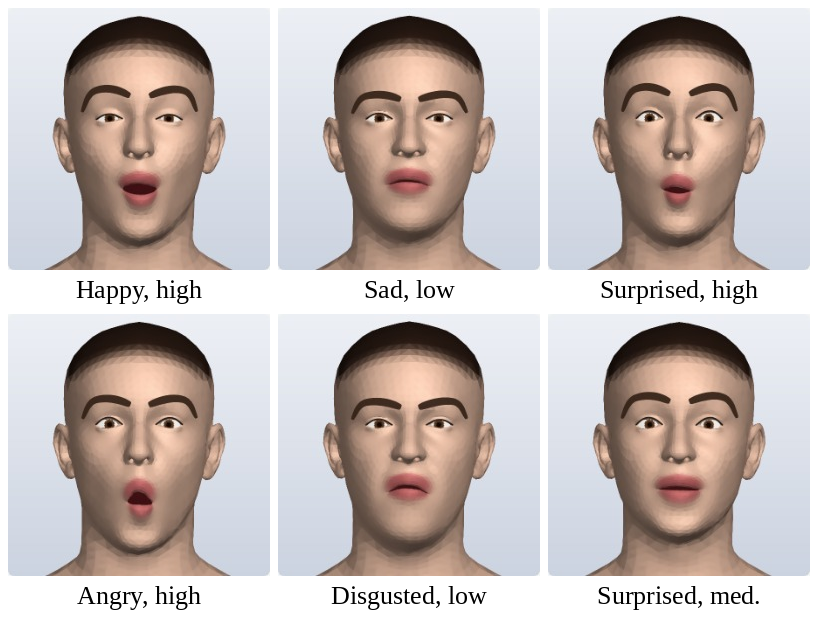
\includegraphics[width=\columnwidth]{fig/emotions.png}
\caption{Our HD renderer on six emotion and intensity settings. Brows, eyelids and mouth shape change with the emotion code.}
\label{fig:emotions}
\end{figure}

\begin{figure}[t]
\centering
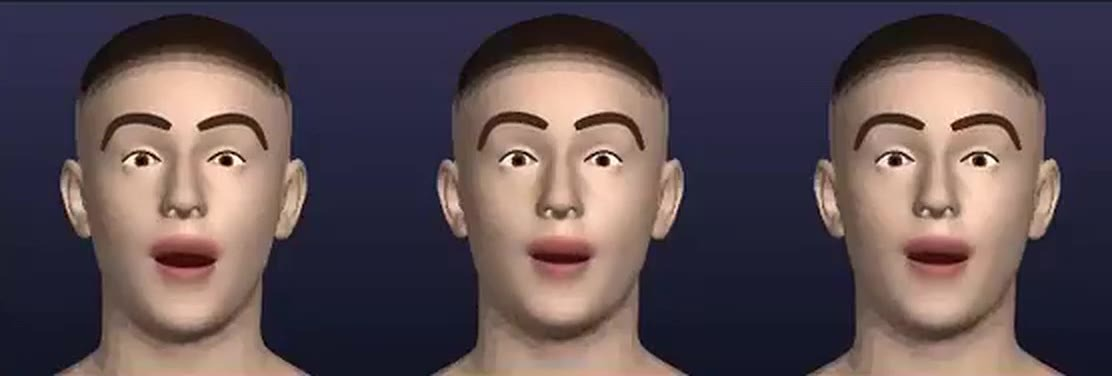
\includegraphics[width=\columnwidth]{fig/takes.jpg}
\caption{Three takes of the same input (speaker M005, surprised, high, $T{=}0.2$) generated in one studio request. Only the codebook sampling differs.}
\label{fig:takes}
\end{figure}

\section{Evaluation}
\label{sec:eval}
\subsection{Ground truth}
We downloaded MEAD audio and the matching 3DMEAD FLAME sequences, converted audio to 16\,kHz, paired every clip and verified all labels. The authors' metric code holds all predictions in memory, which exceeded our hardware, so we wrote \texttt{eval\_stream.py}, which computes the same six metrics incrementally. We evaluated 478 test sequences (57{,}715 frames) from 8 of the 32 test speakers (M003, M009, M013, M023, W009, W011, W014, W016), with 10 samples per sequence at $T{=}0.2$. Table~\ref{tab:gt} compares the results with the paper's Table~1.

\begin{table}[t]
\centering\small
\caption{Our deployment vs.\ the paper on 3DMEAD ground truth ($T{=}0.2$, 10 samples; paper scaling: MVE $\times10^{-3}$, LVE/MEE/CE $\times10^{-4}$, FDD $\times10^{-5}$, diversity $\times10^{-3}$).}
\label{tab:gt}
\begin{tabular}{@{}lccr@{}}
\toprule
Metric & Paper & Ours & Diff.\\
\midrule
MVE $\downarrow$ & 0.7243 & 0.7056 & $-2.6\%$\\
LVE $\downarrow$ & 0.6040 & 0.6417 & $+6.2\%$\\
MEE $\downarrow$ & 0.5549 & 0.5918 & $+6.7\%$\\
CE $\downarrow$ & 0.5227 & 0.5688 & $+8.8\%$\\
FDD $\downarrow$ & 0.0415 & 0.0537 & $+29.3\%$\\
Diversity $\uparrow$ & 0.3274 & 0.3116 & $-4.8\%$\\
\bottomrule
\end{tabular}
\end{table}

MVE and diversity are within 5\% of the published values, and LVE, MEE and CE within 9\%. FDD differs more in relative terms, but its absolute values are tiny (about $5\times10^{-7}$ before scaling), and our subset covers only a quarter of the test speakers, so we read the gap as subset variance rather than a regression.

\subsection{Temperature matrix}
To see what the temperature trades, we repeated the evaluation on the same 478 sequences with sampling off and at four temperatures (Table~\ref{tab:matrix}, Fig.~\ref{fig:tradeoff}). Deterministic decoding has the lowest error and, by construction, zero diversity. At $T{=}0.2$ the vertex error rises by only 1.5\% while diversity reaches 0.31, and MEE and CE are the best of all settings. At $T{=}1.0$ diversity is 2.5 times higher than at $0.2$, but vertex error is 1.8 times the deterministic value. A small amount of randomness helps and a large amount hurts, which supports the paper's choice of $0.2$.

\begin{table}[t]
\centering\small
\caption{Temperature matrix on the same 478 sequences (paper scaling as in Table~\ref{tab:gt}). Best value per column in bold.}
\label{tab:matrix}
\setlength{\tabcolsep}{4pt}
\begin{tabular}{@{}lcccccc@{}}
\toprule
Setting & MVE & LVE & MEE & CE & FDD & Div.\\
\midrule
Sampling off & 0.6955 & 0.6364 & 0.6364 & 0.6364 & \textbf{0.0465} & 0.0000\\
$T{=}0.05$ & \textbf{0.6951} & \textbf{0.6346} & 0.6219 & 0.5968 & 0.0468 & 0.1526\\
$T{=}0.2$ & 0.7056 & 0.6417 & \textbf{0.5918} & \textbf{0.5688} & 0.0537 & 0.3116\\
$T{=}0.5$ & 0.8537 & 0.8059 & 0.6556 & 0.6406 & 0.0863 & 0.5800\\
$T{=}1.0$ & 1.2837 & 1.4393 & 1.1878 & 1.0340 & 0.1142 & \textbf{0.7893}\\
\bottomrule
\end{tabular}
\end{table}

\begin{figure}[t]
\centering
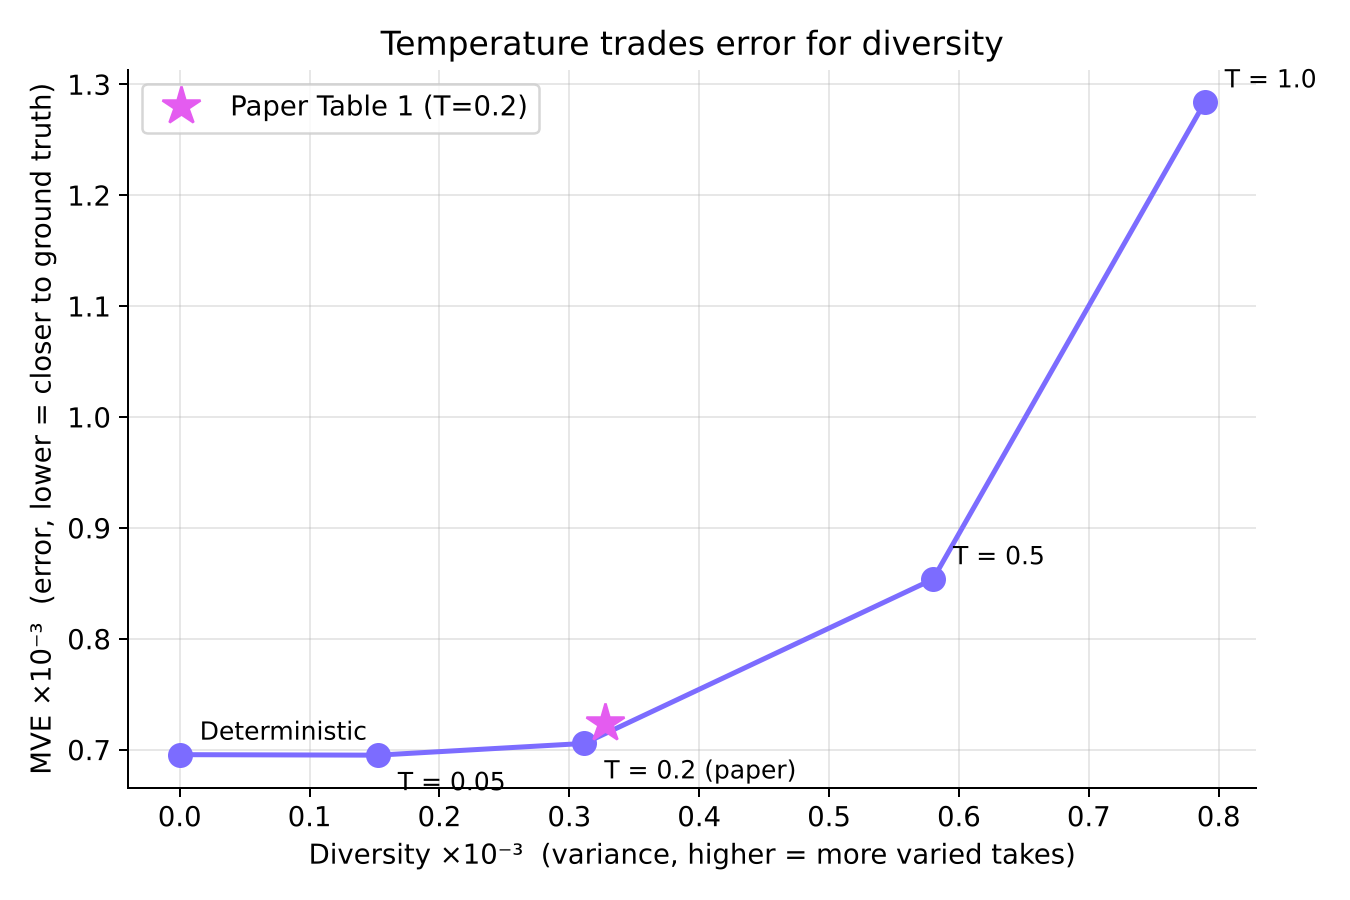
\includegraphics[width=0.92\columnwidth]{fig/tradeoff.png}
\caption{Error against diversity for each temperature setting on the same clips. The paper's Table~1 point (star) lies on our curve near $T{=}0.2$.}
\label{fig:tradeoff}
\end{figure}

\subsection{Where each emotion moves the face}
We fixed a neutral sentence, speaker M009 and high intensity, disabled sampling, generated all eight emotions, and measured the per-vertex displacement from the neutral result (Fig.~\ref{fig:heat}, Table~\ref{tab:disp}). Happy moves the mouth most strongly relative to its whole-face change (4.56\,mm mean mouth displacement). Disgusted produces the largest change overall (5.43\,mm at the mouth, 2.05\,mm in the upper face and up to 8.83\,mm at a single vertex), and angry, disgusted, contempt and sad all move the brows. Surprised and fear produce the smallest changes. Emotion control therefore corresponds to large, region-specific geometric differences rather than a uniform offset.

\begin{figure}[t]
\centering
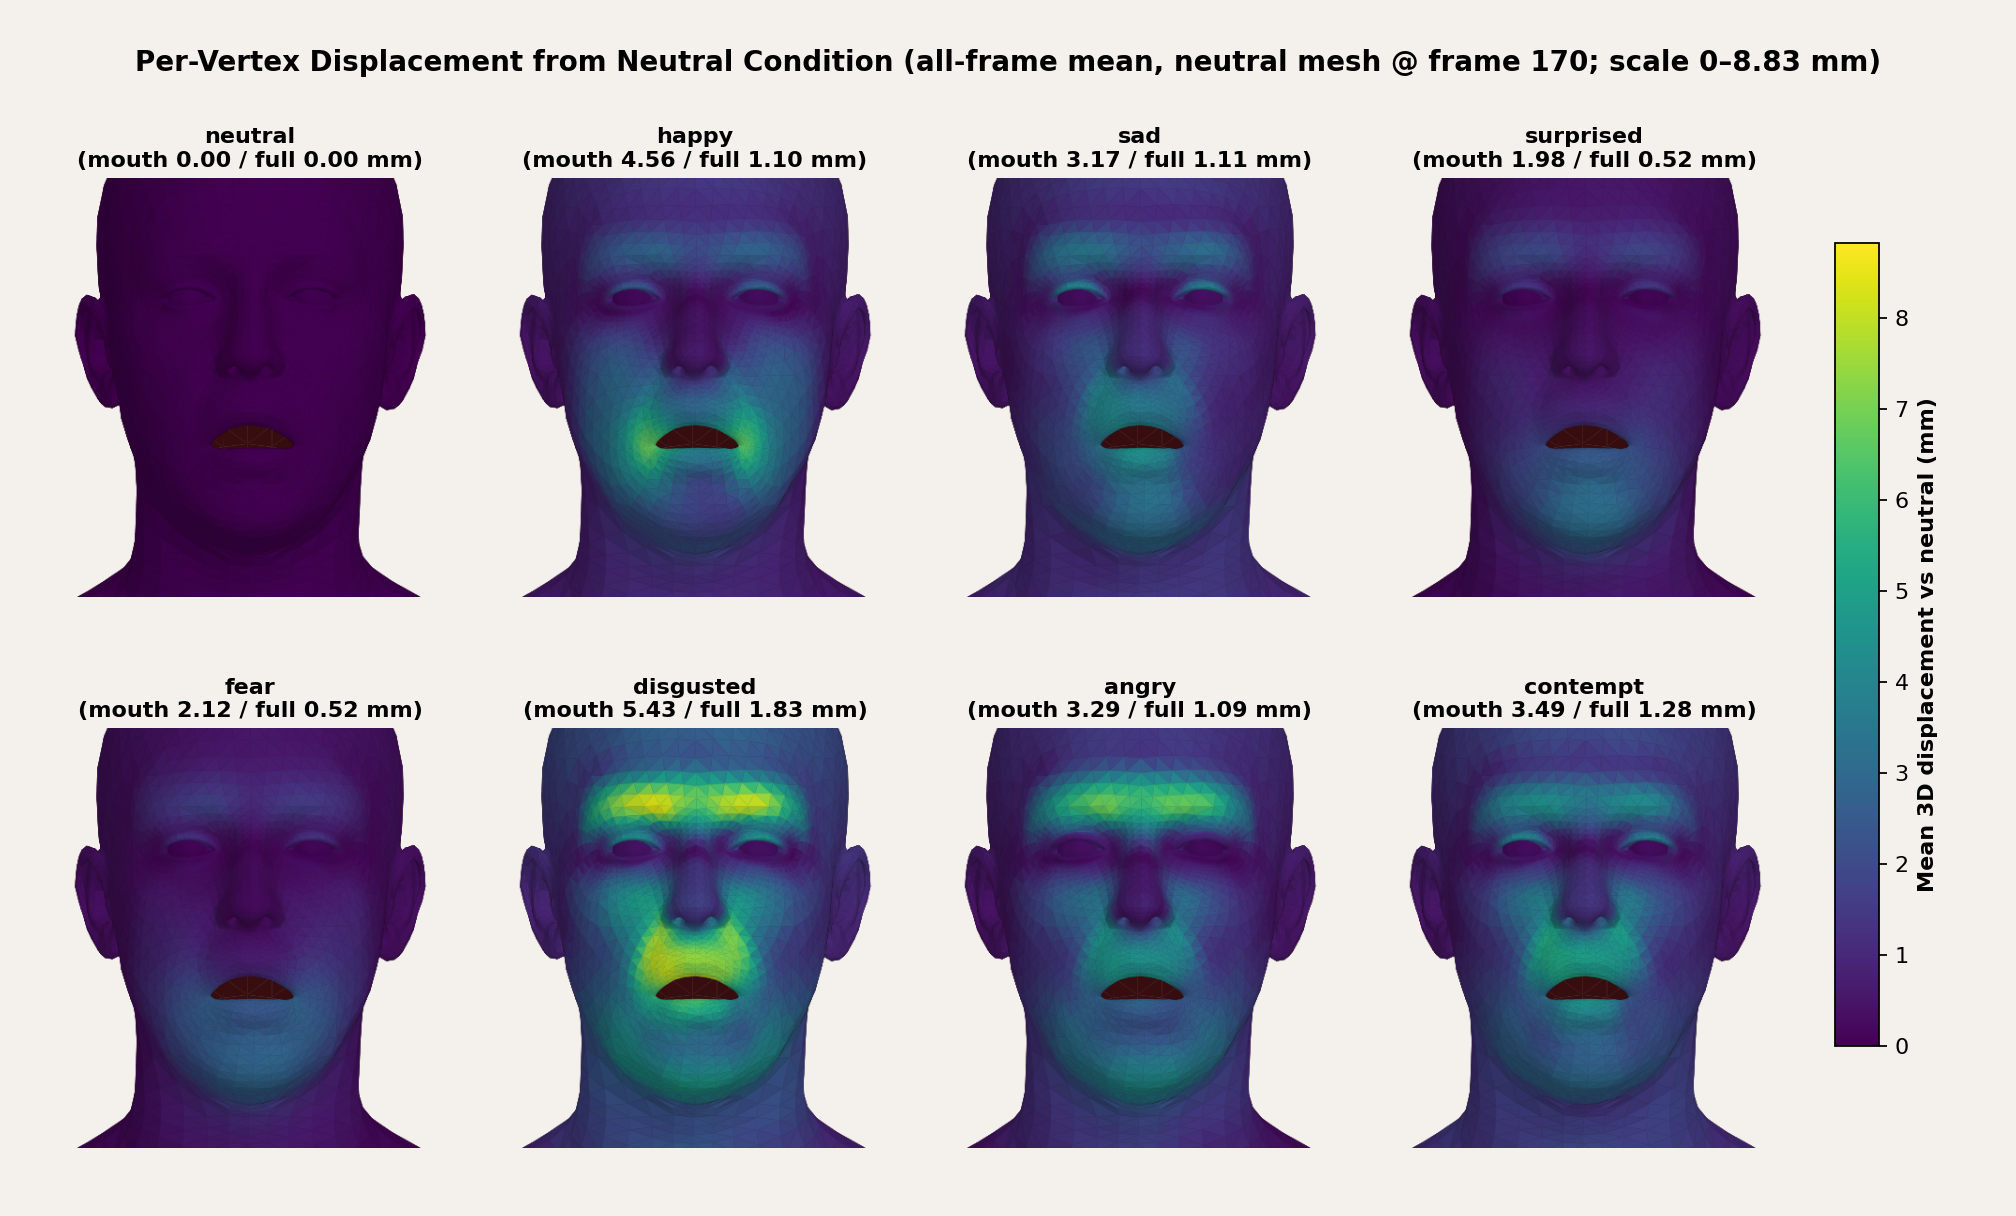
\includegraphics[width=\columnwidth]{fig/heatmaps.png}
\caption{Mean per-vertex displacement from the neutral result for each emotion (speaker M009, high intensity, sampling off).}
\label{fig:heat}
\end{figure}

\begin{table}[t]
\centering\small
\caption{Displacement from neutral in millimetres (mean over frames).}
\label{tab:disp}
\begin{tabular}{@{}lcccc@{}}
\toprule
Emotion & Mouth & Upper face & Whole face & Max vertex\\
\midrule
Happy & 4.56 & 0.95 & 1.10 & 6.87\\
Sad & 3.17 & 1.23 & 1.11 & 4.71\\
Surprised & 1.98 & 0.49 & 0.52 & 3.27\\
Fear & 2.12 & 0.41 & 0.52 & 2.94\\
Disgusted & \textbf{5.43} & \textbf{2.05} & \textbf{1.83} & \textbf{8.83}\\
Angry & 3.29 & 1.26 & 1.09 & 7.26\\
Contempt & 3.49 & 1.49 & 1.28 & 5.61\\
\bottomrule
\end{tabular}
\end{table}

\subsection{User study}
We ran an anonymous Google Form with 25 respondents (64\% a little familiar with 3D animation, games or CGI, 24\% very familiar, 12\% not at all). It contained twelve short clips rendered by our system: four with sound, rated 1--5 for lip-sync and naturalness; six silent clips, each generated with one emotion, where respondents chose one of eight emotions and rated clarity; and two pairs of side-by-side takes, one produced with sampling (different takes) and one an identical control.

\begin{table}[t]
\centering\small
\caption{User study results ($n{=}25$).}
\label{tab:survey}
\begin{tabular}{@{}lc@{}}
\toprule
Measure & Result\\
\midrule
Lip-sync (1--5, 4 clips) & 3.91\\
Naturalness (1--5, 4 clips) & 3.50\\
Emotion accuracy, silent clips (chance 12.5\%) & 38.7\%\\
\quad sad / happy / surprised & 60\% / 52\% / 44\%\\
\quad angry / disgusted / fear & 36\% / 24\% / 16\%\\
Sampled pair judged different & 15/25\\
Identical control judged identical & 13/25\\
\bottomrule
\end{tabular}
\end{table}

Table~\ref{tab:survey} and Fig.~\ref{fig:survey} summarise the results. Lip-sync was rated clearly positive. Naturalness was lower, which we attribute mainly to the untextured, stylised face rather than the motion; one respondent singled out the surprised clip as looking odd. Emotion was recognised from silent clips at 38.7\%, about three times chance; sad and happy were easiest. The main confusions were fear read as surprise (60\%) and disgust read as anger (48\%). These are pairs that share brow and eye configurations and are confused in human perception as well. Detecting take-to-take variation was harder: 15 of 25 respondents saw the sampled pair as different, but 12 of 25 also reported differences in the identical control. Variation at $T{=}0.2$ is therefore subtle at the clip lengths we used, which matches its small effect on vertex error.

\begin{figure}[t]
\centering
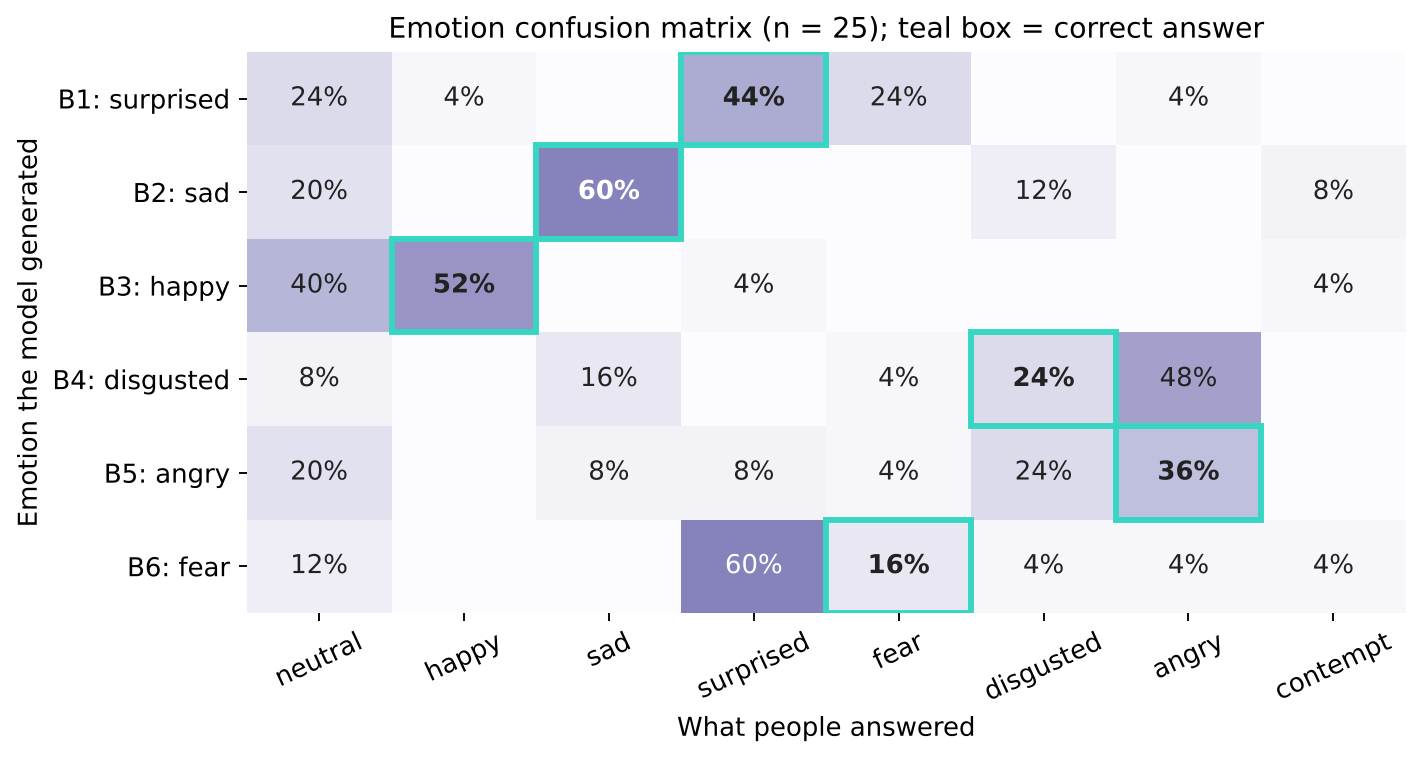
\includegraphics[width=\columnwidth]{fig/survey_confusion.png}
\caption{Emotion confusion on silent clips ($n{=}25$). Boxes mark the correct answer.}
\label{fig:survey}
\end{figure}

\section{Discussion and Limitations}
Our results support the paper's main claims on a modern software stack. Sampling is the sole source of variation, temperature controls it smoothly, and the published accuracy is reproduced within a few percent on real data. Several limitations apply. We evaluated 8 of the 32 test speakers rather than the full set. We used the authors' pretrained weights and did not retrain (an optional HPC training task was not completed). Our renderer has no skin texture or realistic hair, which lowers perceived naturalness and may reduce emotion recognition. CPU rendering, not the model, limits interactive latency, so a GPU or a client-side renderer would be the natural next step. Finally, the user study is small, unpaid and recruited informally, and uses a single neutral sentence per emotion.

\section{Conclusion}
We traced, replicated, deployed and evaluated ProbTalk3D. Three loading patches were enough to run the released model on current software. A Blender-free renderer and a Hugging Face Space turned it into a usable service with web, API and phone clients. Ground-truth metrics, a temperature sweep, displacement maps and a 25-person study together show that the model delivers controllable emotion and controllable variety, and that the paper's default temperature is a sound trade-off between them.

\section*{Author Contributions}
\small
Both authors studied the paper, carried out the Milestone 1 code review and the Milestone 2 replication together, and co-presented the final presentation. \textbf{Jyothi Masina} built the Milestone 3 service (engine, Gradio studio and API, Docker Space, private weight hosting and phone installation), wrote the NumPy FLAME implementation and HD renderer, the streaming ground-truth evaluation and the temperature matrix, designed and analysed the user study, and built the project page. \textbf{Shruti Deulgaonkar} presented the paper background and the first two milestones in the final presentation, distributed the user study and ran the phone demonstration.

\section*{Acknowledgements}
We thank Sichun Wu, Kazi Injamamul Haque and Zerrin Yumak for releasing ProbTalk3D's code and weights. FLAME is used under its own licence and is not redistributed. We used Claude (Anthropic) and the Antigravity coding agent as assistants for planning, code drafting, debugging and writing; all experiments were run and all numbers checked by the authors.

\begin{thebibliography}{99}\small
\setlength{\itemsep}{1pt}
\bibitem{probtalk3d} S.~Wu, K.~I.~Haque and Z.~Yumak. ProbTalk3D: Non-deterministic emotion controllable speech-driven 3D facial animation synthesis using VQ-VAE. In \emph{Proc.\ ACM SIGGRAPH Conference on Motion, Interaction and Games (MIG)}, 2024. \url{https://doi.org/10.1145/3677388.3696320}
\bibitem{vqvae} A.~van den Oord, O.~Vinyals and K.~Kavukcuoglu. Neural discrete representation learning. In \emph{NeurIPS}, 2017.
\bibitem{hubert} W.-N.~Hsu, B.~Bolte, Y.-H.~H.~Tsai, K.~Lakhotia, R.~Salakhutdinov and A.~Mohamed. HuBERT: Self-supervised speech representation learning by masked prediction of hidden units. \emph{IEEE/ACM Trans.\ Audio, Speech, and Language Processing}, 29, 2021.
\bibitem{flame} T.~Li, T.~Bolkart, M.~J.~Black, H.~Li and J.~Romero. Learning a model of facial shape and expression from 4D scans. \emph{ACM Trans.\ Graphics (SIGGRAPH Asia)}, 36(6), 2017.
\bibitem{mead} K.~Wang et al. MEAD: A large-scale audio-visual dataset for emotional talking-face generation. In \emph{ECCV}, 2020.
\bibitem{emote} R.~Dan\v{e}\v{c}ek, K.~Chhatre, S.~Tripathi, Y.~Wen, M.~J.~Black and T.~Bolkart. Emotional speech-driven animation with content-emotion disentanglement. In \emph{SIGGRAPH Asia}, 2023.
\bibitem{voca} D.~Cudeiro, T.~Bolkart, C.~Laidlaw, A.~Ranjan and M.~J.~Black. Capture, learning, and synthesis of 3D speaking styles. In \emph{CVPR}, 2019.
\bibitem{faceformer} Y.~Fan, Z.~Lin, J.~Saito, W.~Wang and T.~Komura. FaceFormer: Speech-driven 3D facial animation with transformers. In \emph{CVPR}, 2022.
\bibitem{codetalker} J.~Xing, M.~Xia, Y.~Zhang, X.~Cun, J.~Wang and T.-T.~Wong. CodeTalker: Speech-driven 3D facial animation with discrete motion prior. In \emph{CVPR}, 2023.
\bibitem{facediffuser} S.~Stan, K.~I.~Haque and Z.~Yumak. FaceDiffuser: Speech-driven 3D facial animation synthesis using diffusion. In \emph{Proc.\ ACM SIGGRAPH MIG}, 2023.
\bibitem{emotalk} Z.~Peng et al. EmoTalk: Speech-driven emotional disentanglement for 3D face animation. In \emph{ICCV}, 2023.
\bibitem{gradio} A.~Abid, A.~Abdalla, A.~Abid, D.~Khan, A.~Alfozan and J.~Zou. Gradio: Hassle-free sharing and testing of ML models in the wild. arXiv:1906.02569, 2019.
\end{thebibliography}

\end{document}
